\section{Results}
For evaluation of the tool, I created simple RISC processor in Scalpel and explored the design space of number of threads (1 - 4), number of pipeline stages (1 - 4), and fixed vs dynamic interleave. The base RISC processor is a classic RISC machine that contains a ICache with a miss latency of 4 cycles, which is accessed through a Variable Latency Interface, and a magic single cycle DMem. 

In order to evaluate how effective the generated multi-threaded designs are at hiding the latencies of long latency functional units in general, which is one of the primary advantages of multi-threading, the ICache is made to pseudo randomly miss based on the output of a LFSR. Each thread accesses its own private ICache through the Variable Latency Unit Interface. This gives a representative evaluation of multi-threaded design effectiveness regardless of the quality of the benchmark program used on the RISC processor.

The metric for performance used is Throughput/Area, which can be broken down into $Task/Cycle * (Cycle/Time)/Area$. $Task/Cycle$ and $(Cycle/Time)/Area$ separately are shown separately from the overall Throughput{\tt /}Area for each design point. Cycle counts are obtained from running an arithmetic benchmark on each design point in Chisel's cycle accurate C++ simulator.

\subsection{Dynamic Interleave}
The trends shown in Figure \ref{fig:dynamicTaskPerCycle}. are generally expected. Task per cycle increases as the number of threads increases due to fewer data dependency hazards and masking of ICache miss latency. Task per cycle decreases as the number of pipeline stages increases beyond the number of threads because the pipeline becomes over saturated and the threads beging to interfere with each other.

The trends shown in Figure \ref{fig:dynamicFreqPerArea}. are also generally expected. $(Cycle/Time)/Area$ decreases as number of threads increase because adding more threads increases the area and increase the critical path length. $(Cycle/Time)/Area$ remains mostly constant as number of pipeline stages because pipeling increases area and decreases the critical path length at the same time.

Multiplying Figure \ref{fig:dynamicTaskPerCycle}. and \ref{fig:dynamicThroughputPerArea}. togther, we obtain Figure \ref{fig:dynamicThroughputPerArea}. From this figure, we can see that the 1 thread, 1 stage designs obtains the best overall Throughput/Area. This is probably because the ICache used in these designs does have have a long enough miss penalty to justify the additional costs of multi-threading.

\subsection{Fixed Interleave}
Because the fixed interleave policy stalls the entire pipeline whenever a Variable Latency Unit Interface signals Resp Pending, the number of threads and number of pipeline stages makes a negligible impact on Task per cycle as shown in \ref{fig:fixedTaskPerCycle}.

Figure \ref{fig:fixedFreqPerArea}. shows that the $(Cycle/Time)/Area$ statistics are very similar to the $(Cycle/Time)/Area$ statistics for dynamic interleave. This tells us that the additional control logic required by dynamic interleave plays a negligible role in determining area and delay.

Multiplying Figure \ref{fig:fixedTaskPerCycle}. and \ref{fig:fixedThroughputPerArea}. togther, we obtain Figure \ref{fig:fixedThroughputPerArea}. From this figure, we can see that the 1 thread, 1 stage designs obtains the best overall Throughput/Area just like with dynamic interleave. However, all of the design points have lower Throughput/Area than their equivalents with dynamic interleave. Thus, we can conclude that for the example RISC processor design, the latency benefits gained from dynamic interleave outweigh the additional area and delay cost of the more complex control logic in dynamic interleave.

\begin{figure}
\centering
\resizebox{\columnwidth}{!}{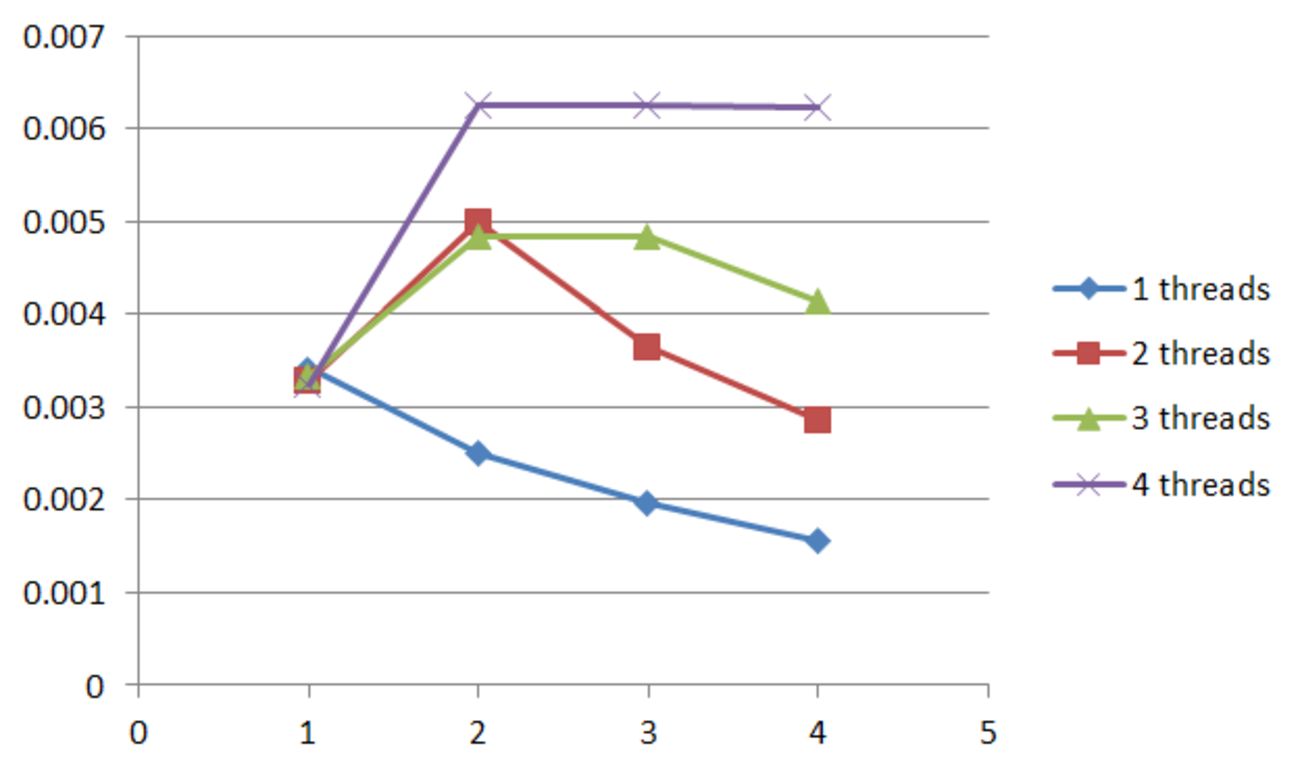
\includegraphics{figures/DynamicTaskPerCycle.pdf}}
\caption{{\bf Dynamic Interleave Task{\tt /}Cycle} The Y-Axis is in units of $task/cycle$.}
\label{fig:dynamicTaskPerCycle}
\centering
\resizebox{\columnwidth}{!}{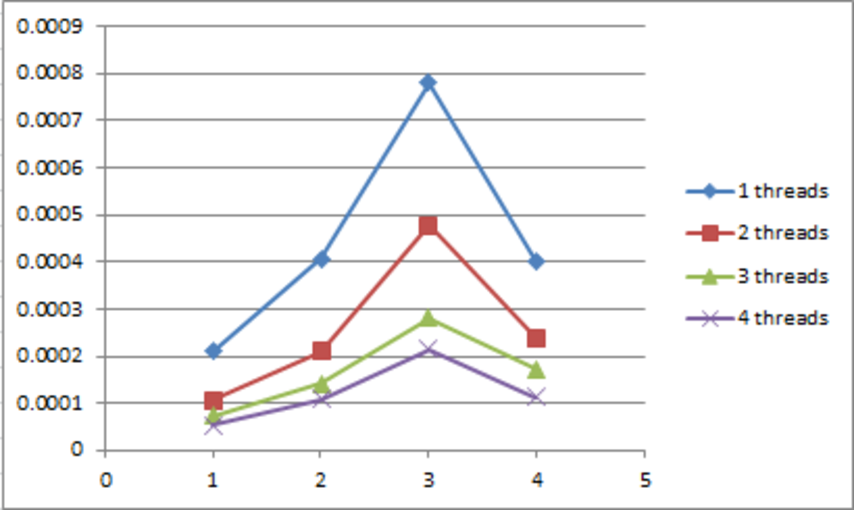
\includegraphics{figures/DynamicFreqPerArea.pdf}}
\caption{{\bf Dynamic Interleave (Cycle{\tt /}Time){\tt /}Area} The Y-Axis is in units of $GHz/um^2$.}
\label{fig:dynamicFreqPerArea}
\centering
\resizebox{\columnwidth}{!}{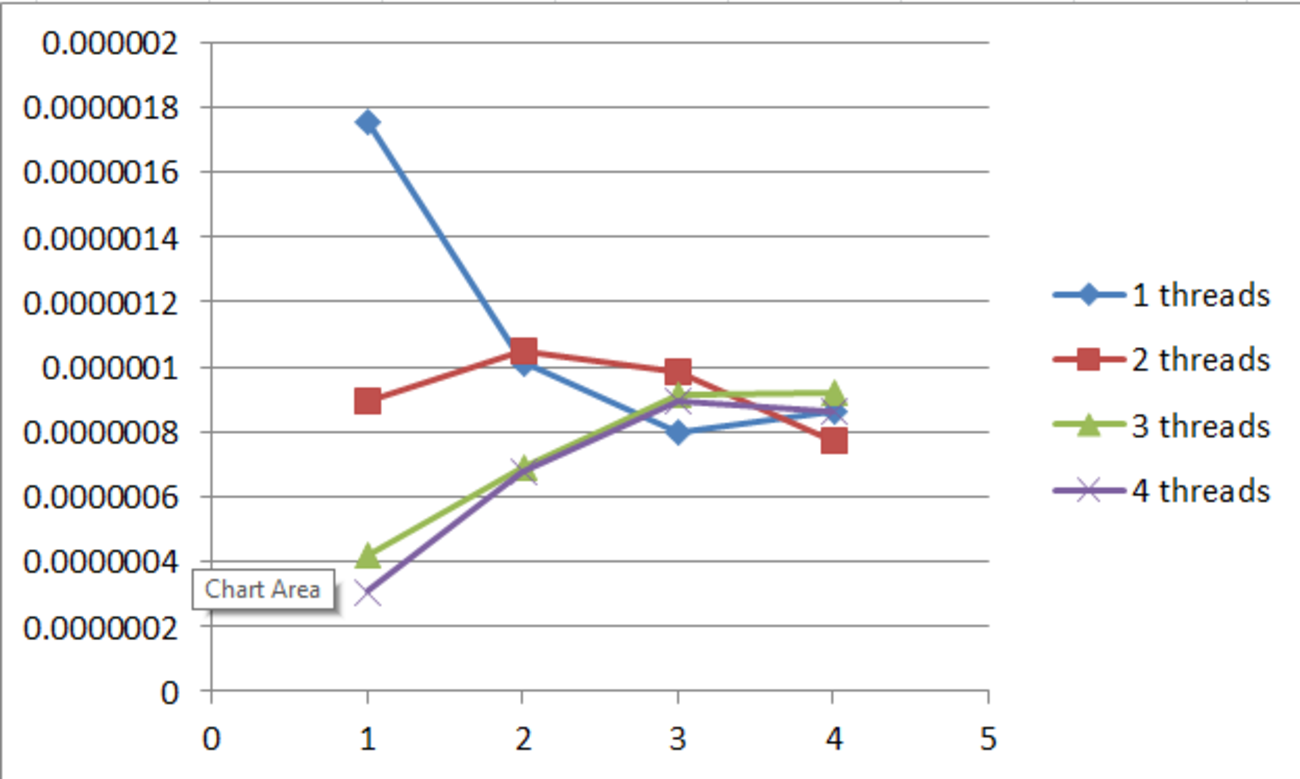
\includegraphics{figures/DynamicThroughputPerArea.pdf}}
\caption{{\bf Dynamic Interleave Throughput{\tt /}Area} The Y-Axis is in units of $(task/ns)/um^2$.}
\label{fig:dynamicThroughputPerArea}
\end{figure}

\begin{figure}
\centering
\resizebox{\columnwidth}{!}{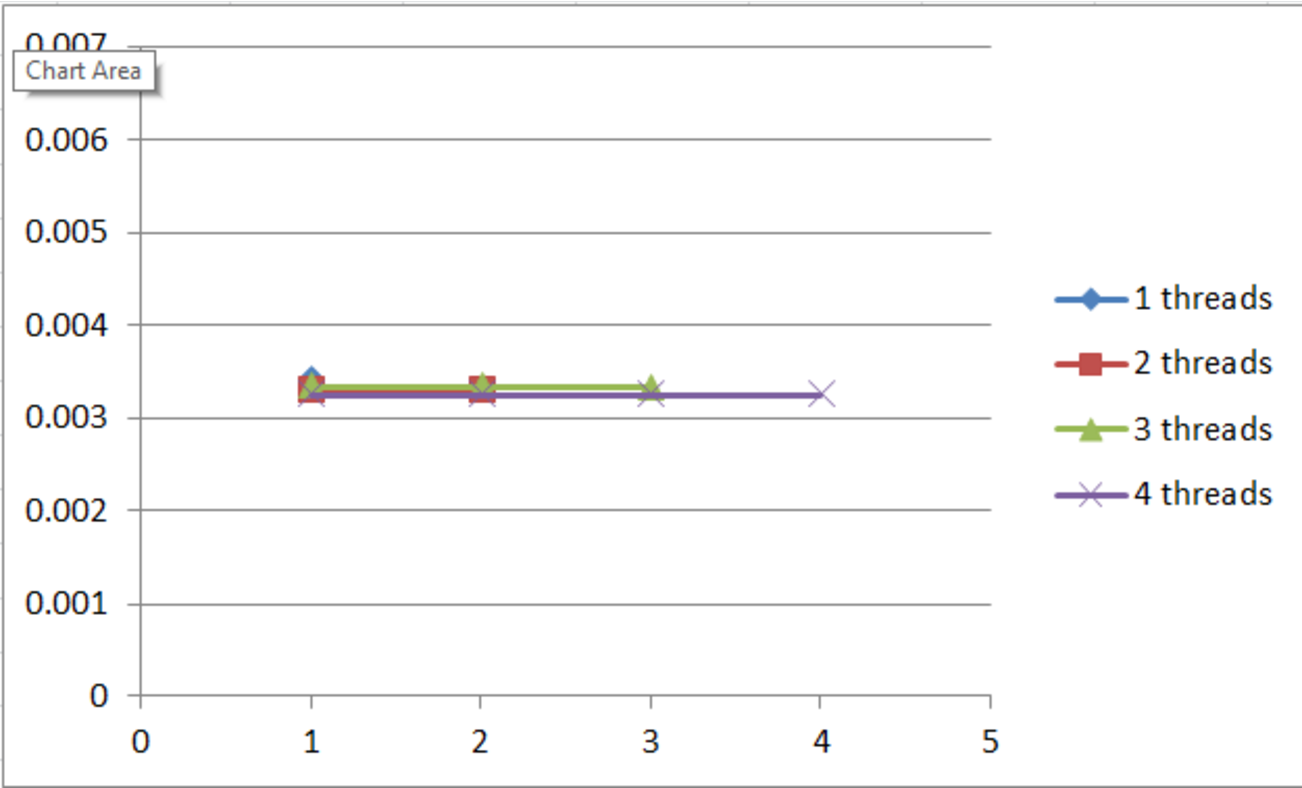
\includegraphics{figures/FixedTaskPerCycle.pdf}}
\caption{{\bf Fixed Interleave Task{\tt /}Cycle} The data points where number of stages {\tt >} number of threads are not valid design points for fixed interleave, so they do not exist on this chart. The Y-Axis is in units of $task/cycle$.}
\label{fig:fixedTaskPerCycle}
\centering
\resizebox{\columnwidth}{!}{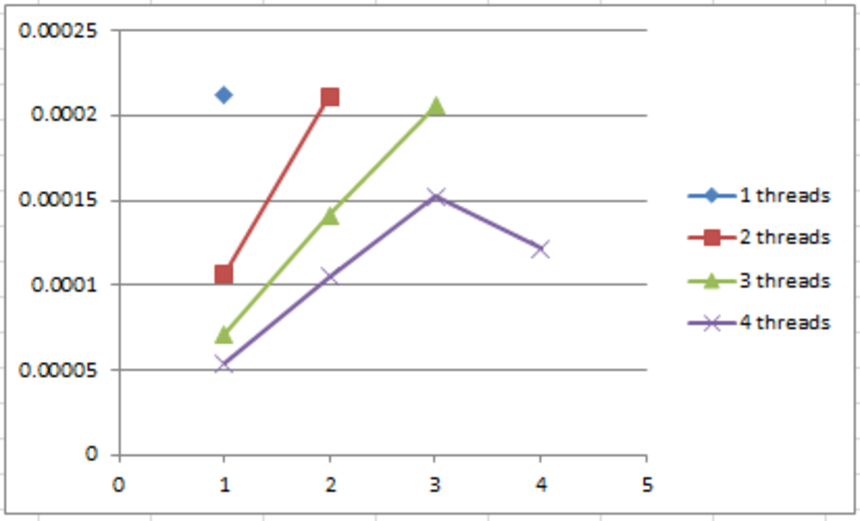
\includegraphics{figures/FixedFreqPerArea.pdf}}
\caption{{\bf Fixed Interleave (Cycle{\tt /}Time){\tt /}Area} The data points where number of stages {\tt >} number of threads are not valid design points for fixed interleave, so they do not exist on this chart. The Y-Axis is in units of $GHz/um^2$.}
\label{fig:fixedFreqPerArea}
\centering
\resizebox{\columnwidth}{!}{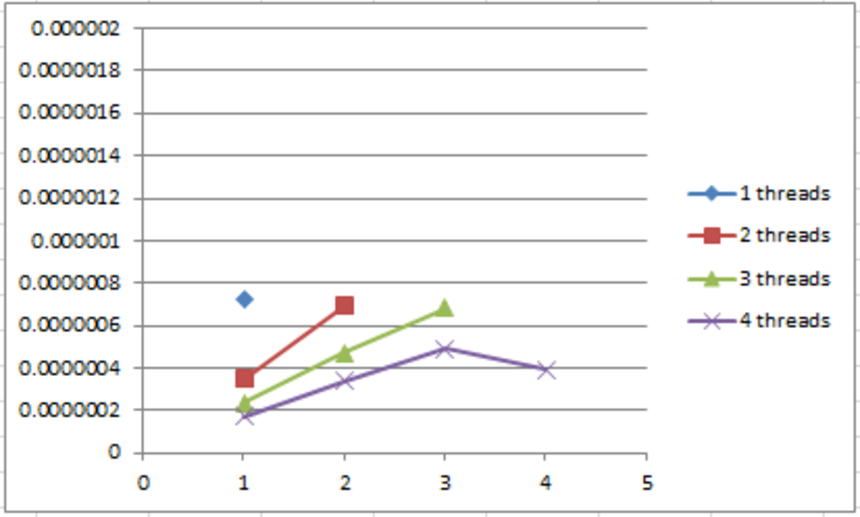
\includegraphics{figures/FixedThroughputPerArea.pdf}}
\caption{{\bf Fixed Interleave Throughput{\tt /}Area} The data points where number of stages {\tt >} number of threads are not valid design points for fixed interleave, so they do not exist on this chart. The Y-Axis is in units of $(task/ns)/um^2$.}
\label{fig:fixedThroughputPerArea}
\end{figure}



